\begin{pastexam}[label={px:ccu-115-swa-07}]{中正資工所甲組 115 學年度 第 17 題}
（複選；全對才給分）

(2\%) (\qquad) For determining the articulation points in the following graph, list the depth-first search
numbers (starting from 1) for each vertex in the order of $A, B, C, D, E, F, G, H,$ and $I$. Begin
the depth-first search at \textbf{vertex $A$}. If multiple unvisited vertices are available during
the search, select the vertex with the smallest alphabetical label.
\begin{center}
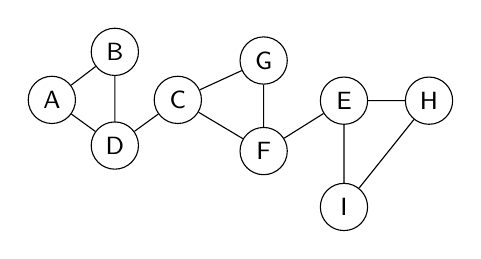
\begin{tikzpicture}[x=1cm,y=1cm,v/.style={circle,draw,minimum size=6mm,inner sep=1pt,font=\small\sffamily}]
\node[v] (A) at (0.75,-1.17) {A};
\node[v] (B) at (1.55,-0.56) {B};
\node[v] (D) at (1.55,-1.75) {D};
\node[v] (C) at (2.35,-1.17) {C};
\node[v] (G) at (3.44,-0.67) {G};
\node[v] (F) at (3.44,-1.82) {F};
\node[v] (E) at (4.46,-1.18) {E};
\node[v] (H) at (5.54,-1.18) {H};
\node[v] (I) at (4.46,-2.53) {I};
\draw (A)--(B) (A)--(D) (B)--(D) (D)--(C) (C)--(G) (C)--(F) (G)--(F) (F)--(E) (E)--(H) (E)--(I) (H)--(I);
\end{tikzpicture}
\end{center}
(a)~(1, 2, 3, 4, 5, 6, 7, 8, 9) \qquad (b)~(1, 9, 3, 2, 6, 5, 4, 8, 7)\\
(c)~(1, 2, 4, 3, 7, 6, 5, 8, 9) \qquad (d)~(1, 2, 4, 3, 6, 5, 9, 7, 8)\\
(e)~none of the above
\end{pastexam}

\begin{pastsoln}
答案：(d)。

邊是 A--B、A--D、B--D、C--D、C--F、C--G、F--G、E--F、E--H、E--I、H--I。 從 A 做 DFS，每次從目前
頂點挑字母最小的未拜訪鄰居（資結書第~21.4~節）；沒有就退回上一層。 $d$ 是拜訪的順序：
\begin{center}
\small
\begin{tabular}{cll}
\toprule
$d$ & 拜訪 & 說明 \\
\midrule
1 & A & 起點；鄰居 B、D \\
2 & B & A 的鄰居裡最小的 \\
3 & D & B 的鄰居 A 已拜訪，只剩 D \\
4 & C & D 的鄰居 A、B 已拜訪，剩 C \\
5 & F & C 的鄰居 F、G，取 F \\
6 & E & F 的鄰居 C 已拜訪，E、G 取 E \\
7 & H & E 的鄰居 H、I 取 H \\
8 & I & H 的鄰居 E 已拜訪，剩 I \\
9 & G & I 沒有新鄰居，退回 H、E 也沒有，退回 F，剩 G \\
\bottomrule
\end{tabular}
\end{center}
依 A, B, \ldots, I 的順序寫出 $d$：$(1, 2, 4, 3, 6, 5, 9, 7, 8)$，就是 (d)。

DFS 樹的樹邊是 A--B、B--D、D--C、C--F、F--E、E--H、H--I、F--G；其餘三條 A--D、G--C、I--E 是後向邊。
\begin{itemize}
\item (a) 錯：把字母順序當成拜訪順序，但 B 之後走到的是 D（C 和 B 不相鄰）。
\item (b) 錯：B 應該是第 $2$ 個，不是第 $9$ 個。
\item (c) 錯：E、F、G 的編號錯。 C 之後先走 F（字母比 G 小），不是 G。
\item (e) 錯，(d) 對。
\end{itemize}
\end{pastsoln}
